% \documentclass{beamer}
\documentclass[8pt]{beamer}

\usetheme{Madrid} % 기본 테마, 다른 테마 사용 가능
\usefonttheme[onlymath]{serif}
\usefonttheme{professionalfonts}
% 테마 선택 (선택 사항)
% \font{serif}
\usepackage{amsfonts}
\usepackage{amssymb}
\usepackage{graphicx}  % 이미지 삽입 패키지


% \setcounter{MaxMatrixCols}{20}

% (필요한 패키지들)
% \usepackage{amsthm}
\setbeamertemplate{theorems}[numbered]  % 정리, 정의 등에 번호를 달아줌

% \theoremstyle{plain} % insert bellow all blocks you want in italic
% \newtheorem{theorem}{Theorem}[section] % to number according to section
% 
% \theoremstyle{definition} % insert bellow all blocks you want in normal text
% \newtheorem{definition}{Definition}[section] % to number according to section
% \newtheorem*{idea}{Proof idea} % no numbered block
\usepackage{tcolorbox}

% 필요할 경우 패키지 추가
\usepackage{graphicx} % 이미지 삽입을 위한 패키지
\usepackage{amsmath}   % 수식 사용
\usepackage{hyperref}  % 하이퍼링크 추가
\usepackage{cleveref}
\usepackage{multicol}  % 여러 열 나누기


\newcommand{\mrm}[1]{\mathrm{#1}}
\newcommand{\mbb}[1]{\mathbb{#1}}
\newcommand{\mb}[1]{\mathbf{#1}}
\newcommand{\mc}[1]{\mathcal{#1}}
\newcommand{\tb}[1]{\textbf{#1}}
\newcommand{\ti}[1]{\textit{#1}}

% \setbeamerfont{math text}{size=\tiny}
% \setbeamerfont{math text inlined}{size=\tiny}
% \setbeamerfont{math text display}{size=\small}
% \setbeamerfont{math text display}{size=\tiny}
% \setbeamerfont{math text display}{size=\scriptsize}
% \setbeamerfont{math text display}{size=\tiny}




% 발표 제목, 저자, 날짜 설정
\title{Soft Actor-Critic}
\author{Gwanwoo Choi}
% \date{}

\begin{document}

\begin{frame}
    \titlepage
\end{frame}


\begin{frame}{RL with Maximum Entropy Objective}
State value function $V$, action value function $Q$, and RL objective function $J(\pi)$ can be newly defined in maxiumum entropy augmented RL frameworks.

\bigskip

    \begin{itemize}
        \item \(
            Q^\pi_\text{soft}(s_t, a_t) \triangleq r(s_t,a_t) + \gamma \mathbb{E}_{s_{t+1} \sim P}[V^\pi_\text{soft}(s_{t+1})]
            \)
        \item \(
            V^\pi_\text{soft}(s_t) \triangleq \mathbb{E}_{a_t \sim \pi}[Q^\pi_\text{soft} (s_t,a_t)] + \mathcal{H}(\pi (\cdot | s_t))
            \)
        \item \(J(\pi) \triangleq \sum_{t=0}^\infty \mathbb{E}_{(s_t,a_t) \sim d^\pi} [Q^\pi_\text{soft} (s_t, a_t) + \alpha \mathcal{H}(\pi(\cdot | s_t))]
        \)
    \end{itemize}

\bigskip
With these definition, completely new version of Policy Iteration algorithm can be derived. Iteratively repeat under algorithms
\begin{itemize}
    \item Soft Policy Evaluation
    \item Soft Policy Improvement
\end{itemize}
leads to \textbf{Soft Policy Iteration}.

\end{frame}

\begin{frame}{Soft Policy Improvement}
Let assume tabular setting first. For arbitrary policy \(\pi\), there exists soft value functions and \(V^\pi_\text{soft} (s), \forall s\) and $Q^\pi_\text{soft}(s, a), \forall s, a$.

\bigskip

\begin{theorem}[\textbf{Soft Policy Improvement}]
    Consider about another policy \(\pi^\prime \in \Pi\) such that \(\pi^\prime(a|s) \propto \exp{(Q^\pi_\text{soft}(s, a))} \). Then
    \(Q^{\pi^\prime}_\text{soft}(s,a) \geq Q^{\pi}_\text{soft}(s,a), \forall (s,a) \in \mathcal{S}\times\mathcal{A}\).
\end{theorem}

To proof soft policy improvement theorem, we first see another lemma.

\end{frame}

\begin{frame}{Soft Policy Improvement}
    For the simplicity of proof, \(\alpha = 1\) is assumed.

    \begin{lemma}
        \[
            \mathbb{E}_{a \sim \pi}[Q^\pi_\text{soft}(s, a)] + \mathcal{H}(\pi(\cdot | s)) \leq \mathbb{E}_{a \sim \pi^\prime}[Q^{\pi}_\text{soft}(s, a)] + \mathcal{H}(\pi^\prime(\cdot | s)), \forall s \in \mathcal{S}
        \]
    \end{lemma}
    \textit{Proof.} Recall the fact that \(\pi^\prime(a|s) = \frac{\exp{(Q^\pi_\text{soft} (s, a))}}{\sum_{a^\prime} \exp{(Q^\pi_\text{soft} (s, a^\prime))}}\).
    First, let's modify the RHS.
    \[\begin{aligned}
        &\mathbb{E}_{a \sim \pi^\prime}[Q^\pi_\text{soft}(s,a)] + \mathcal{H}(\pi^\prime(\cdot | s)) = \mathbb{E}_{a \sim \pi^\prime} [Q^\pi_\text{soft}(s,a) - \log{\pi^\prime (a|s)}]\\
        = &\mathbb{E}_{a \sim \pi^\prime}[\log{\sum_{a^\prime}\exp{(Q^\pi_\text{soft}(s,a^\prime))}}] = \log{\sum_{a^\prime}\exp{(Q^\pi_\text{soft}(s, a^\prime))}} 
    \end{aligned}
    \]

    \smallskip

    And, consider about the LHS. By the fact $D_\text{KL}(p \parallel q) = \mathcal{H}(p, q) - \mathcal{H}(p)$, \[\begin{aligned}
        &\mathbb{E}_{a \sim \pi}[Q^\pi_\text{soft}(s,a)] + \mathcal{H}(\pi(\cdot |s)) = \mathbb{E}_{a\sim \pi}[Q^\pi_\text{soft}(s,a)] + \mathcal{H}(\pi(\cdot | s), \pi^\prime(\cdot | s)) - D_{\text{KL}}(\pi(\cdot |s)\parallel \pi^\prime (\cdot | s)) \\ =& \mathbb{E}_{a \sim \pi}[Q^\pi_\text{soft}(s,a) - \log{\pi^\prime(a|s)}] - D_{\text{KL}}(\pi(\cdot | s)\parallel \pi^\prime(\cdot |s)) \\ 
        = &\mathbb{E}_{a \sim \pi}[\log{\sum_{a^\prime}}\exp{(Q^\pi_\text{soft}(s,a^\prime))}] - D_\text{KL}(\pi(\cdot |s\parallel \pi^\prime (\cdot | s))) \\= &\log{\sum_{a^\prime}\exp{(Q^\pi_\text{soft}(s,a^\prime))}}- D_{\text{KL}}(\pi(\cdot | s\parallel \pi^\prime(\cdot | s)))
    \end{aligned}
    \]
    Since, for any probability density function $p, q$,  $D_{\text{KL}}(p \parallel q) \geq 0$ holds, LHS $\leq$ RHS.
\end{frame}

\begin{frame}{Soft Policy Improvement}
    \begin{block}{Theorem 1 (\textbf{Soft Policy Improvement})}
        Consider about another policy \(\pi^\prime \in \Pi\) such that \(\pi^\prime(a|s) \propto \exp{(Q^\pi_\text{soft}(s, a))} \). Then
        \(Q^{\pi^\prime}_\text{soft}(s,a) \geq Q^{\pi}_\text{soft}(s,a), \forall (s,a) \in \mathcal{S}\times\mathcal{A}\).
    \end{block}

    \textit{Proof.} Repeatedly roll out $Q^\pi_\text{soft}$ and adjust lemma 2 forever. Then result of theorem 1 is obtained.
    \[
    \begin{aligned}
        &Q^\pi_\text{soft}(s_t,a_t), \forall (s_t,a_t) \in \mathcal{S}\times \mathcal{A} \\
        &= r(s_t,a_t) + \gamma \mathbb{E}_{s_{t+1}} [\mathcal{H}(\pi(\cdot | s_{t+1})) + \mathbb{E}_{a_{t+1} \sim \pi}[Q^\pi_\text{soft}(s_{t+1}, a_{t+1})]] \\
        &\leq r(s_t, a_t) + \gamma \mathbb{E}_{s_{t+1}}[\mathcal{H}(\pi^\prime (\cdot | s_{t+1})) + \mathbb{E}_{a_{t+1}\sim \pi^\prime}[Q^\pi_\text{soft}(s_{t+1}, a_{t+1})]] \\
        &\leq r(s_t, a_t) + \gamma \mathbb{E}_{s_{t+1}}[\mathcal{H}(\pi^\prime( \cdot| s_{t+1})) + \mathbb{E}_{a_{t+1}\sim \pi^\prime} [r(s_{t+1}, a_{t+1}) + \gamma \mathbb{E}_{s_{t+2}}[\mathcal{H}(\pi^\prime(\cdot | s_{t+2})) + \dots]]]
        \\
        &\vdots \\
        &\leq Q^{\pi^\prime}_{\text{soft}}(s_t,a_t)
    \end{aligned}
    \]

\end{frame}

\begin{frame}{Soft Policy Evaluation}
    From now on, $Q^\pi_\text{soft}$ and $V^\pi_\text{soft}$ are briefly denoted as $Q^\pi$ and $V^\pi$.
    \newline

    For simplicity of proof, let me introduce entropy augmedted reward, $r_\pi(s_t, a_t) \triangleq r(s_t,a_t) + \gamma \mathbb{E}_{s_{t+1}}[\mathcal{H}(\pi(\cdot | s_{t+1}))]$.

    Let define soft bellman operator for any $Q: \mathcal{S}\times \mathcal{A} \mapsto \mathbb{R}$, $(\mathcal{T}^\pi Q) (s_t,a_t) \triangleq r_\pi(s_t,a_t) + \gamma \mathbb{E}_{s_{t+1}}[\mathbb{E}_{a_{t+1}}[ Q(s_{t+1}, a_{t+1})]]$.

    \begin{theorem}[\textbf{Soft Policy Evaluation}]
        Let $\mathcal{Q}: \{Q \mid Q: \mathcal{S}\times\mathcal{A} \mapsto \mathbb{R} \}$. For arbitrary $Q \in \mathcal{Q}$,
        $((\mathcal{T}^\pi)^k Q) \rightarrow Q^\pi$ as $k \rightarrow \infty$. 
        

        % \[
        % || \mathcal{T}^\pi Q^1 - \mathcal{T}^\pi Q^2 || \leq \gamma || Q^1 - Q^2||
        % \]
        % holds.
    \end{theorem}
    \textit{Proof.}
        Define distance  between $Q^1$ and $Q^2$ as $||Q^1 - Q^2|| \triangleq \max_{s^\prime, a^\prime} |Q^1(s^\prime,a^\prime) - Q^2(s^\prime, a^\prime)|$.
        Then
        \(||(\mathcal{T}^\pi Q) - Q^\pi|| = ||(\mathcal{T}^\pi Q)- (\mathcal{T}^\pi Q^\pi)|| = \max_{s^\prime, a^\prime} \left| r_\pi(s^\prime,a^\prime) - r_\pi(s^\prime, a^\prime) + \gamma \mathbb{E}_{s_{t+1}, a_{t+1}}[(Q(s_{t+1}, a_{t+1}) - Q^\pi(s_{t+1}, a_{t+1}))] \right| \leq \gamma \max_{s^\prime, a^\prime} \vert Q(s^\prime, a^\prime) - Q^\pi(s^\prime, a^\prime) \vert\).

        This implies that \( \Vert ((\mathcal{T}^\pi)^k Q) - Q^\pi \Vert \leq \gamma^k \Vert Q - Q^\pi \Vert \) and as \( k \rightarrow \infty\), \((\mathcal{T}^\pi)^\infty Q \rightarrow Q^\pi\).

\end{frame}

\begin{frame}{Soft Policy Iteration}
    \begin{theorem}[Soft Policy Iteration]
        Repeated application of soft evaluation and soft policy improvement to any $\pi \in \Pi$ converges to a policy $\pi^\prime$ such that $Q^{\pi^\prime} (s_t, a_t) \geq Q^\pi (s_t, a_t)$ for all $\pi \in \Pi$ and $(s_t, a_t) \in \mathcal{S}\times\mathcal{A}$
    \end{theorem}
    Let denote $k$-th updated policy as $\pi_k$. Then $Q^{\pi_k}$ is bounded above for $\pi^\ast \in \Pi$ and it converges to $Q^{\pi^\ast}$. Also, $Q^{\pi^\ast} (s,a) \geq Q^{\pi_k} (s,a)$ for any $\pi_k \in \Pi, (s,a) \in \mathcal{S} \times \mathcal{A}$ by policy improvement theorem. So, iteratively adapt policy evaluation and policy improvement leads to optimal policy $\pi^\ast$ and optimal value function $Q^{\pi^\ast}$.
    \bigskip

    Now Soft Policy Iteration algorithm can be described as
    \begin{itemize}
        \item Initialize arbitrary policy $\pi$
        \item Evaluate $Q^\pi$
        \item Construct new policy $\pi^\prime$ from $\pi$
        \item While $\pi^\prime$ converges
        \begin{itemize}
            \item $\pi \leftarrow \pi^\prime$
            \item Evaluate $Q^\pi$
            \item Construct new policy $\pi^\prime$ from $\pi$
        \end{itemize}
    \end{itemize}
\end{frame}


\begin{frame}{Soft Policy Iteration with Function Approximation}
    From soft policy iteration algorithm,
    \begin{itemize}
        \item Initialize arbitrary policy $\pi$
        \item Evaluate $Q^\pi$
        \item Construct new policy $\pi^\prime$ from $\pi$
        \item While $\pi^\prime$ converges
        \begin{itemize}
            \item $\pi \leftarrow \pi^\prime$
            \item Evaluate $Q^\pi$
            \item Construct new policy $\pi^\prime$ from $\pi$
        \end{itemize}
    \end{itemize}

    We can parametrize both $\pi$ and $Q^\pi$ In this algorithm.
    $\pi \approx \pi_\phi$ and $Q^{\pi_\phi} \approx Q_\theta$.
    And soft policy iteration algorithm converted to
    \begin{itemize}
        \item Initialize $\phi$, $\theta$ arbitrary (for $\pi_\phi$ and $Q_\theta$)
        \item For each iteration
        \begin{itemize}
            \item For each environment step
            \begin{itemize}
                \item $a_t \sim \pi_\phi(a_t | s_t), s_{t+1} \sim P(s_{t+1}|s_t, a_t)$
                \item $\mathcal{D} \leftarrow \mathcal{D} \cup \{s_t, a_t, r(s_t, a_t), s_{t+1}\}$            
            \end{itemize}
            \item For each gradient step
            \begin{itemize}
                \item update $\theta$ (evalute $Q_\theta$)
                \item update $\phi$  (policy improvement $\pi_\phi$)
            \end{itemize}
        \end{itemize}
    \end{itemize}
\end{frame}

\begin{frame}{Objective Function for Policy Parameter}
    In algorithm, 
    \begin{itemize}
        \item Initialize $\phi$, $\theta$ arbitrary (for $\pi_\phi$ and $Q_\theta$)
        \item For each iteration
        \begin{itemize}
            \item For each environment step
            \begin{itemize}
                \item $a_t \sim \pi_\phi(a_t | s_t), s_{t+1} \sim P(s_{t+1}|s_t, a_t)$
                \item $\mathcal{D} \leftarrow \mathcal{D} \cup \{s_t, a_t, r(s_t, a_t), s_{t+1}\}$            
            \end{itemize}
            \item For each gradient step
            \begin{itemize}
                \item update $\theta$ (evalute $Q_\theta$)
                \item update $\phi$  (policy improvement $\pi_\phi$)
            \end{itemize}
        \end{itemize}
    \end{itemize}


    Recall that update rule of policy in tabular setting is
    \[
        \pi^\prime(a|s) = \frac{\exp{(Q^\pi_\text{soft} (s, a))}}{\sum_{a^\prime} \exp{(Q^\pi_\text{soft} (s, a^\prime))}} = \arg \min_{\pi^\prime \in \Pi} D_\text{KL} \left( \pi^\prime (\cdot|s) \parallel \frac{\exp{(Q^\pi_\text{soft} (s, \cdot))}}{\sum_{a^\prime} \exp{(Q^\pi_\text{soft} (s, a^\prime))}}  \right)
    \]

    update rule for $\phi$ is defined as 
    \[
        J_\pi (\phi) = \mathbb{E}_{s_t \sim \mathcal{D}}\left[D_\text{KL} \left( \pi_\phi (\cdot | s) \parallel \frac{\exp{Q_\theta}(s, \cdot)}{\sum_{a^\prime} \exp{Q_\theta (s, a^\prime)}} \right)\right]
    \]

    We can approximate $\arg \min_{\pi^\prime \in \Pi}$ as gradient descent algorithm.
\end{frame}

\begin{frame}{Objective Function for Policy Parameter}
    \[
        J_\pi (\phi) = \mathbb{E}_{s_t \sim \mathcal{D}}\left[D_\text{KL} \left( \pi_\phi (\cdot | s) \parallel \frac{\exp{(Q_\theta)}(s, \cdot)}{\sum_{a^\prime} \exp{Q_\theta (s, a^\prime)}} \right)\right]
    \]
Reparametrization trick can be applid to this objective function, resulting in a lower variance estimator. Let $a_t = f_\phi (\epsilon_t; s_t)$ sampled action that depends on some random noise like $\epsilon \sim \mathcal{N}(0, I)$. We can sample action by calculating $a_t = \mu_\phi(s_t) + \Sigma_\phi(s_t) \odot \epsilon_t$ in each timestep.

% \[
% \begin{aligned}
    % J_\pi (\phi) &= \mathbb{E}_{s_t \sim \mathcal{D}, \epsilon_t \sim \mathcal{N}}[ \log{\pi_\phi}(f_\phi (\epsilon_t ; s_t)|s_t) - Q_\theta (s_t, f_\phi (\epsilon_t; s_t)) + \log{\sum_{a^\prime} \exp{Q_\theta (s, a^\prime)}}] \\
    % &= \mathbb{E}_{s_t \sim \mathcal{D}, \epsilon_t \sim \mathcal{N}}[ \log{\pi_\phi}(f_\phi (\epsilon_t ; s_t)|s_t) - Q_\theta (s_t, f_\phi (\epsilon_t; s_t))] 
% \end{aligned}
% \]

\[
    J_\pi (\phi) = \mathbb{E}_{s_t \sim \mathcal{D}, \epsilon_t \sim \mathcal{N}}[ \log{\pi_\phi}(f_\phi (\epsilon_t ; s_t)|s_t) - Q_\theta (s_t, f_\phi (\epsilon_t; s_t))]
\]

We can simply drop $\log{\sum_a^\prime \exp{Q_\theta(s,a^\prime)}}$ because this term doesn't modify the gradient $\nabla J_\pi (\phi)$.

Gradient of $\nabla J_\pi (\phi)$ can be estimated by
\[
    \hat{\nabla}_\phi J_\pi (\phi) = \nabla_\phi \log{\pi_\phi (a_t| s_t)} + (\nabla_{a_t} \log{\pi_\phi}(a_t | s_t) - \nabla_{a_t}Q(s_t,a_t))\nabla_\phi f_\phi (\epsilon_t ; s_t)
\]
\end{frame}

\begin{frame}{Objective Function for Value Function Approximator}
    \begin{itemize}
        \item Initialize $\phi$, $\theta$ arbitrary (for $\pi_\phi$ and $Q_\theta$)
        \item For each iteration
        \begin{itemize}
            \item For each environment step
            \begin{itemize}
                \item $a_t \sim \pi_\phi(a_t | s_t), s_{t+1} \sim P(s_{t+1}|s_t, a_t)$
                \item $\mathcal{D} \leftarrow \mathcal{D} \cup \{s_t, a_t, r(s_t, a_t), s_{t+1}\}$            
            \end{itemize}
            \item For each gradient step
            \begin{itemize}
                \item update $\theta$ (evalute $Q_\theta$)
                \item update $\phi$ (\(\phi \leftarrow \phi - \lambda_\pi \hat{\nabla}_\phi J_\pi(\phi)\))
            \end{itemize}
        \end{itemize}
    \end{itemize}

    Recall that \[ Q^\pi (s_t,a_t) = r(s_t,a_t) + \gamma \mathbb{E}_{s_{t+1}} [\mathcal{H}(\pi(\cdot | s_{t+1})) + \mathbb{E}_{a_{t+1}}[Q^\pi (s_{t+1}, a_{t+1})]] \]
    But by using the fact \(V^\pi(s_{t+1}) = \mathcal{H}(\pi(\cdot | s_{t+1})) + \mathbb{E}_{a_{t+1}}[Q^\pi(s_{t+1}, a_{t+1})]\), above equation can be simplified by \[Q^\pi (s_t, a_t) = r(s_t, a_t) + \gamma \mathbb{E}_{s_{t+1}}[V^\pi (s_{t+1})]\]

\end{frame}


\begin{frame}{Objective Function for Value Function Approximator}
    Let introduce state value function estimator $V^\pi \approx V_\psi$.

    From equations,
    \[
    \begin{gathered}
        Q^\pi (s_t, a_t) = r(s_t, a_t) + \gamma \mathbb{E}_{s_{t+1}}[V^\pi (s_{t+1})] \\
        V^\pi(s_{t+1}) = \mathcal{H}(\pi(\cdot | s_{t+1})) + \mathbb{E}_{a_{t+1}}[Q^\pi(s_{t+1}, a_{t+1})]
    \end{gathered}
    \]

    Objective function for each state value function and action value function can be defined by $J_V (\psi)$ and $J_Q (\theta)$.

    \begin{equation*}
        J_V(\psi) = \mathbb{E}_{s_t \sim \mathcal{D}} \left[ \frac{1}{2} \left(V_\psi (s_t) - \mathbb{E}_{a_t \sim \pi_\phi}[Q_\theta(s_t, a_t) - \log{\pi_\phi (a_t | s_t)}]\right)^2 \right] 
    \end{equation*}

    \begin{equation*}
        J_Q(\theta) = \mathbb{E}_{(s_t,a_t) \sim \mathcal{D}} \left[ \frac{1}{2} \left(Q_\theta (s_t, a_t) - r(s_t,a_t) - \gamma \mathbb{E}_{s_{t+1}}[V_{\bar{\psi}}(s_{t+1})] \right)^2\right]
    \end{equation*}

    And the derivative $\hat{\nabla}_\psi$ and $\hat{\nabla}_\theta$ can be estimated by

    \begin{equation*}
        \hat{\nabla}_\psi J_V (\psi) = \nabla_\psi V_\psi (s_t) (V_\psi (s_t) - Q_\theta (s_t, a_t) + \log{\pi_\phi}(a_t|s_t))
    \end{equation*}

    \begin{equation*}
        \hat{\nabla}_\theta J_Q (\theta) = \nabla_\theta Q_\theta (s_t, a_t)(Q_\theta (s_t, a_t) - r(s_t, a_t) - \gamma V_{\bar{\psi}}(s_{t+1}))
    \end{equation*}

    Where the $V_{\bar{\psi}}$ is the seperated network updated with exponential moving average of network parameter $V_\psi$, which stablizes training.
    \[
       \tau \leftarrow \tau \psi + (1- \tau)\bar{\psi}
    \]
\end{frame}

\begin{frame}{Two Q Functions}
    \begin{itemize}
        \item Initialize $\psi, \bar{\psi}, \phi$, $\theta$ arbitrary (for $\pi_\phi$ and $Q_\theta$)
        \item For each iteration
        \begin{itemize}
            \item For each environment step
            \begin{itemize}
                \item $a_t \sim \pi_\phi(a_t | s_t), s_{t+1} \sim P(s_{t+1}|s_t, a_t)$
                \item $\mathcal{D} \leftarrow \mathcal{D} \cup \{s_t, a_t, r(s_t, a_t), s_{t+1}\}$            
            \end{itemize}
            \item For each gradient step
            \begin{itemize}
                \item update $\psi$ (\( \psi \leftarrow \psi - \lambda_V \hat{\nabla}_\psi J_V (\psi) \))
                \item update $\theta$ (\( \theta \leftarrow \theta - \lambda_Q \hat{\nabla}_\theta J_Q (\theta)\))
                \item update $\phi$ (\(\phi \leftarrow \phi - \lambda_\pi \hat{\nabla}_\phi J_\pi(\phi)\))
                \item update $\bar{\psi}$ ($\tau \leftarrow \tau \psi + (1- \tau)\bar{\psi}$)
            \end{itemize}
        \end{itemize}
    \end{itemize}

    Using two Q functions is known to mitigate positive bias in the policy improvement step. So use two Q parameters $\theta_i, \forall i \in \{0, 1\}$. Then $J_\pi (\phi)$ and $J_V (\psi)$ turns to 


    \begin{equation*}
        J_\pi (\phi) = \mathbb{E}_{s_t \sim \mathcal{D}, \epsilon_t \sim \mathcal{N}} [\log{\pi_\phi (f_\phi (\epsilon; s_t)| s_t)} - \min_i Q_{\theta_i} (s_t, f_\phi(\epsilon_t ; s_t)) ]
    \end{equation*}
    \begin{equation*}
        J_V(\psi) = \mathbb{E}_{s_t \sim \mathcal{D}} \left[ \frac{1}{2} \left(V_\psi (s_t) - \mathbb{E}_{a_t \sim \pi_\phi}[\min_i Q_{\theta_i}(s_t, a_t) - \log{\pi_\phi (a_t | s_t)}]\right)^2 \right]
    \end{equation*}

    And each $\theta_i$ is updated separately.

    \[
    \theta_i \leftarrow \theta_i -  \lambda_Q \hat{\nabla}_{\theta_i} J_Q(\theta_i), \forall i
    \]

\end{frame}


\begin{frame}{Soft Actor-Critic}
    Now the final soft actor critic algorithm is

    \begin{itemize}
        \item Initialize $\psi, \bar{\psi}, \phi$, $\theta$ arbitrary (for $\pi_\phi$ and $Q_\theta$)
        \item For each iteration
        \begin{itemize}
            \item For each environment step
            \begin{itemize}
                \item $a_t \sim \pi_\phi(a_t | s_t), s_{t+1} \sim P(s_{t+1}|s_t, a_t)$
                \item $\mathcal{D} \leftarrow \mathcal{D} \cup \{s_t, a_t, r(s_t, a_t), s_{t+1}\}$            
            \end{itemize}
            \item For each gradient step
            \begin{itemize}
                \item update $\psi$ (\( \psi \leftarrow \psi - \lambda_V \hat{\nabla}_\psi J_V (\psi) \))
                \item update $\theta_i, \forall i$ (\( \theta_i \leftarrow \theta_i - \lambda_Q \hat{\nabla}_{\theta_i} J_Q (\theta_i)\))
                \item update $\phi$ (\(\phi \leftarrow \phi - \lambda_\pi \hat{\nabla}_\phi J_\pi(\phi)\))
                \item update $\bar{\psi}$ ($\tau \leftarrow \tau \psi + (1- \tau)\bar{\psi}$)
            \end{itemize}
        \end{itemize}
    \end{itemize}
\end{frame}

\begin{frame}{Code Implementation}
    Choose Walker2D environment, which has continuous state space and continuous action space.

    Network is defined by fully connected layer which has 2 hidden layers. (Following the guideline of Appendix.D)

    \begin{figure}
        \centering
        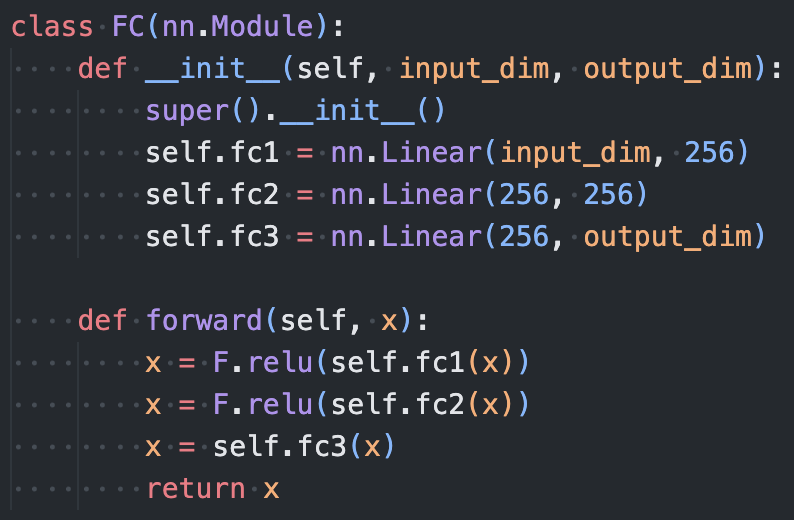
\includegraphics[width=0.3\textwidth]{fig1.png}
        
\includegraphics[width=0.45\textwidth]{fig2.png}
    \end{figure}

    In Walker2D, $a_t$ is bounded in $[-1.0, 1.0]$, so $a_t = \tanh{(\mu_\phi(s_t)+ \Sigma_\phi(s_t) \odot \epsilon_t)}$

    \begin{itemize}
        \item There are some bugs in sample action function
        \item After re-aranging the action value, range of action becomes $[0, 2]$, not $[-1, 1]$
    \end{itemize}
\end{frame}

\begin{frame}{Code Implementation}
    In walker2D, $\vert \mathcal{S} \vert = 17$ and $\vert \mathcal{A} \vert = 6$.

    \begin{itemize}
        \item V network gets $\vert \mathcal{S} \vert$ input and $1$ output
        \item Q network gets $\vert \mathcal{S} \vert + \vert \mathcal{A} \vert$ input and $1$ output
        \item Policy network gets $\vert \mathcal{S} \vert$ input and $2\vert \mathcal{A} \vert$ output, which each of $\vert \mathcal{A} \vert$ means mean and standard deviation of Gaussian
        \item Sampling function of Policy network gets $2 \vert \mathcal{A} \vert$ input and $\vert \mathcal{A} \vert$ output
    
    \end{itemize}

    
    \begin{figure}
        \centering
        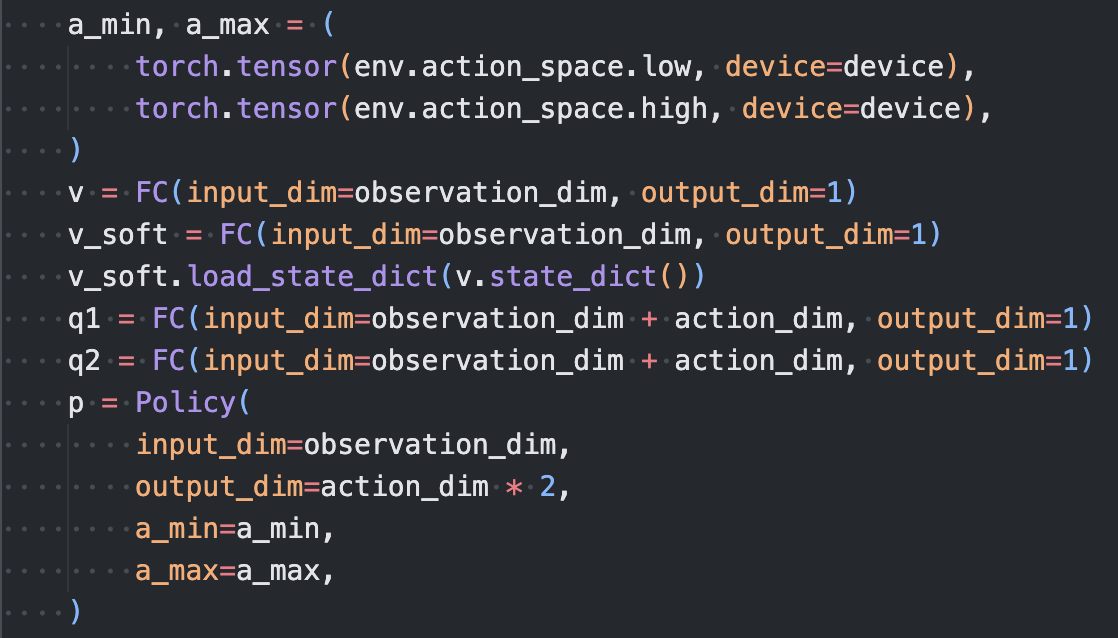
\includegraphics[width=0.4\textwidth]{fig3.png}
        
\includegraphics[width=0.4\textwidth]{fig2.png}
    \end{figure}

\end{frame}

\begin{frame}{Code Implementation}
    \begin{equation*}
        J_V(\psi) = \mathbb{E}_{s_t \sim \mathcal{D}} \left[ \frac{1}{2} \left(V_\psi (s_t) - \mathbb{E}_{a_t \sim \pi_\phi}[\min_i Q_{\theta_i}(s_t, a_t) - \log{\pi_\phi (a_t | s_t)}]\right)^2 \right]
    \end{equation*}
    \begin{equation*}
        J_Q(\theta) = \mathbb{E}_{(s_t,a_t) \sim \mathcal{D}} \left[ \frac{1}{2} \left(Q_\theta (s_t, a_t) - r(s_t,a_t) - \gamma \mathbb{E}_{s_{t+1}}[V_{\bar{\psi}}(s_{t+1})] \right)^2\right]
    \end{equation*}
    \begin{figure}
        \centering
        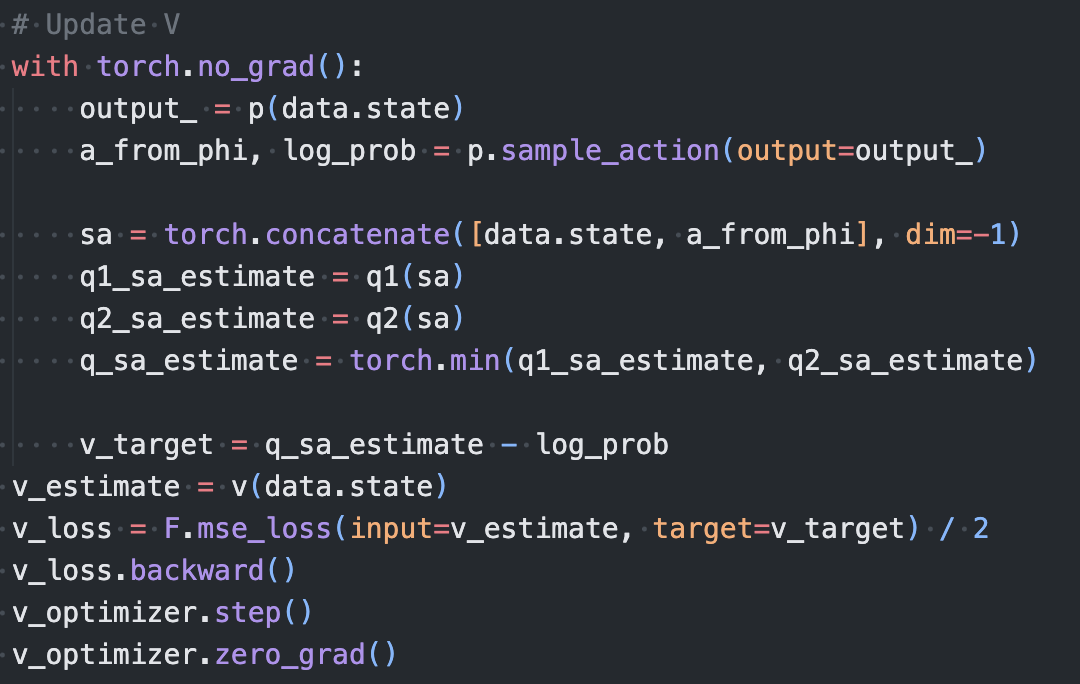
\includegraphics[width=0.45\textwidth]{fig4.png}
        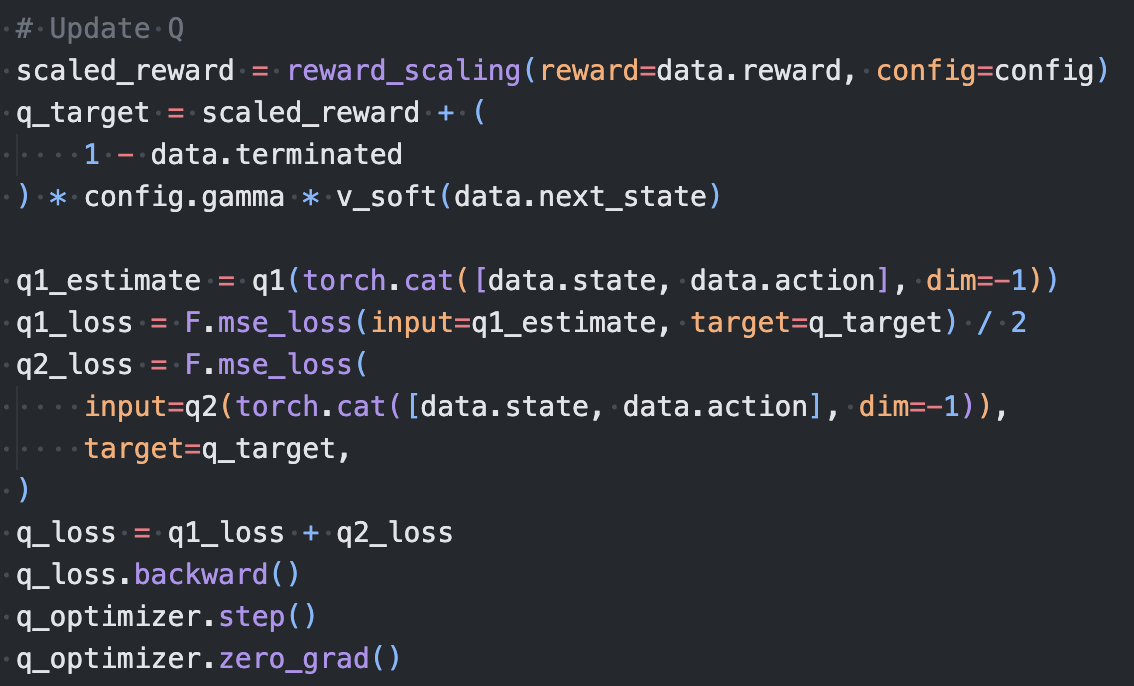
\includegraphics[width=0.45\textwidth]{fig5.png}
    \end{figure}

    \begin{itemize}
        \item Also, there exists bug in calculating $Q_1$ and $Q_2$ loss
        \item $Q_1$ loss is 2 times smaller than $Q_2$ loss
    \end{itemize}
\end{frame}

\begin{frame}{Code Implementation}
    \begin{equation*}
        J_\pi (\phi) = \mathbb{E}_{s_t \sim \mathcal{D}, \epsilon_t \sim \mathcal{N}} [\log{\pi_\phi (f_\phi (\epsilon; s_t)| s_t)} - \min_i Q_{\theta_i} (s_t, f_\phi(\epsilon_t ; s_t)) ]
    \end{equation*}
    \[
        \tau \leftarrow \tau \psi + (1- \tau)\bar{\psi}
     \]
    \begin{figure}
        \centering
        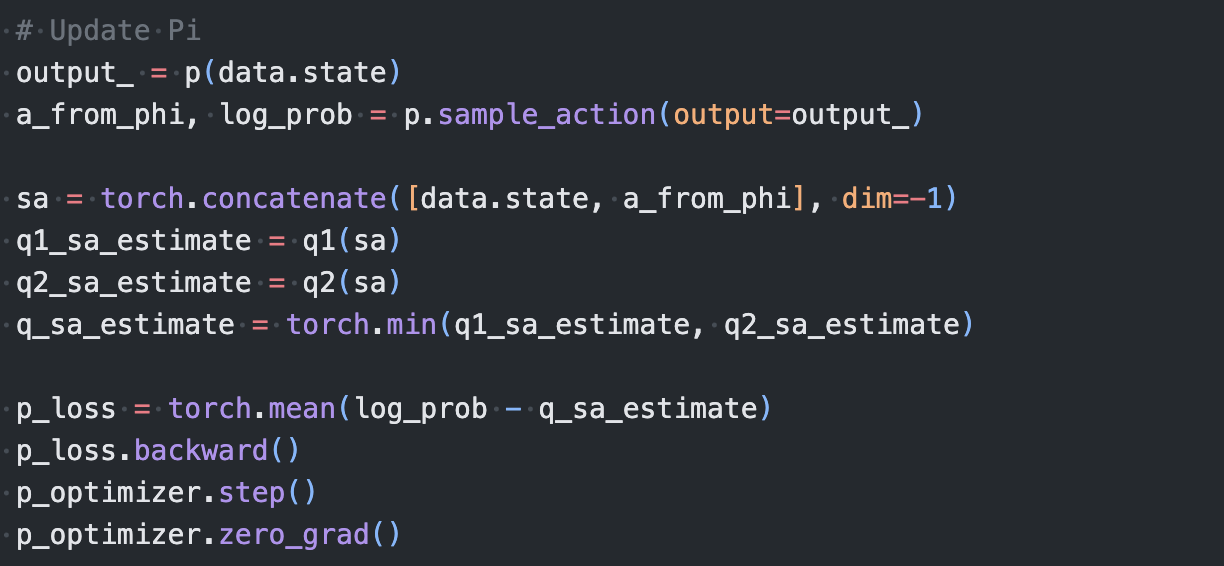
\includegraphics[width=0.45\textwidth]{fig6.png}
        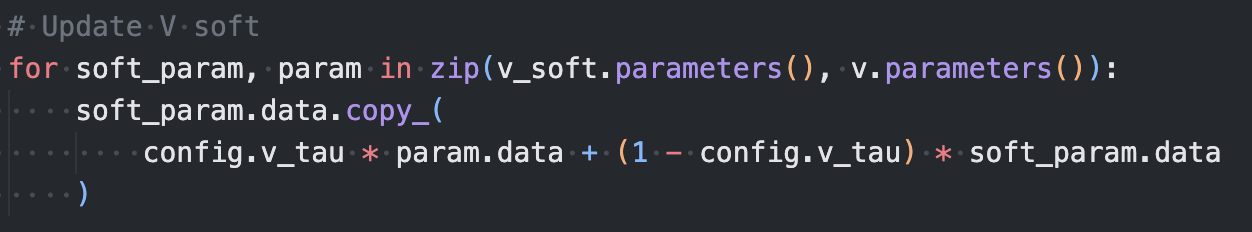
\includegraphics[width=0.45\textwidth]{fig7.png}
    \end{figure}
\end{frame}

\end{document}